\documentclass{article}
\author{Jakub Daszewski \and Dawid S. Jakubczyk}
\title{Obiektowy projekt systemu informatycznego w notacji UML}
\date{25.05.26 r. Uniwesrytet Warmińsko-Mazurski, Olsztyn}
\usepackage{polski}
\usepackage[table]{xcolor}
\usepackage[a4paper, margin=1in]{geometry}
\usepackage{hyperref}
\usepackage{fancyhdr}
\usepackage{ragged2e}
\usepackage{graphicx}
\renewcommand{\baselinestretch}{1.15} 
\pagenumbering{arabic}
\begin{document}
	\pagestyle{fancy}
	\begin{titlepage}
	\maketitle
	\center Ver. 1.0.1
	\center \textbf{Projektowanie Systemów Informatycznych}
	\center \textbf{Prowadzący: mgr inż. A. Samojluk} \\
	\end{titlepage}
	\tableofcontents
	\newpage
	\fancyhead[R]{Daszewski, Jakubczyk}
	\fancyhead[L]{System Zarządzanie Katalogami}
	\section{Analiza Biznesowa}	
	\justify \textbf{Dziedzina Problemowa: }Problem który rozwiązuje system informatyczny to zarządzanie wyposażeniem, układanie terminarza wizyt, pomoc w obsłudze wizyty\\
	\justify \textbf{Opis Organizacji: }Organizacja dla ktorej Si jest przeznaczony to średniej wielkosci przychodnia medyczna która obsługuje około 150 osób w ciagu dnia
	

\subsection*{Obsługa wizyt, łącznie z zarządzaniem pacjentami i lekarzami.}

\subsubsection*{Kontekst dziedziny problemowej:}

\justify Pacjent przychodzi do rejestracji rejestrujac sie na wizyte, przychodnia rezerwuje gabinet lekarski, czas lekarza, i jesli jest wymagany sprzet medyczny to rowniez jest przypisywany do wizyty. Po wizycie publicznej NFZ rozlicza sie z przychodnia, jesli wizyta byla prywatna pacjent reguluje naleznosci w rejestracji.
Przychodnia odpowiada za przeslanie informacji do systemu recept.
 
\subsubsection*{Procesy i aktorzy biznesowi:}

\begin{tabular}{|m{6em}|m{10em}|m{18em}|m{7em}|}
\hline
\rowcolor{lightgray} Proces & Aktor Biznesowy & Funkcje/zadania & Dane\\
\hline
Rejestracja Pacjenta	& Pacjent\newline pracownik rejestracji & Pracownik rejestracji ustala wizyte z lekarzem & Dane Pacjenta, Informacje medyczne\\
\hline
Sprawdzanie dostępności & Pracownik & Prawcownik sprawdza dostępność lekarzy & Kalendzarz robczy lekarza\\
\hline
\end{tabular}
\newpage
\subsection*{Zarządzanie wyposażeniem przychodni, łącznie z obsługą zakupu i instalacji wyposażenia.}

\subsubsection*{Kontekst dziedziny problemowej:}
System monitoruje stany wyposażenia i udostepnia informacje o stanie gdy jest to konieczne, system opracowuje też terminy przeglądów i powiadamia jeśli coś wymaga przeglądu
\subsubsection*{Procesy i aktorzy biznesowi:}
\begin{tabular}{|m{6em}|m{10em}|m{18em}|m{7em}|}
	\hline
	\rowcolor{lightgray} Proces & Aktor Biznesowy & Funkcje/zadania & Dane\\
	\hline
	Zakup nowego wyposażenia & Producent Wyposażenia &- Pracownik przychodni  kupuję i wprowadza nowe wyposażenie do bazy danych & Dowód zakupu\\
	\hline
	Instalacja nowego wyposażenia & Firma Instalacyjna &- Przychodnia wynajmuję firmę zajmującą się instalacją nowego wyposażenia medycznego \newline- Pracownik wynajętej firmy instaluje nowe wyposażenie \newline- przychondnia opłaca wynajętą firmę & Faktura \\
	\hline
	Okresowy przegląd wyposażenia & Firma Konserwacyjna &- Pracownik konserwacyjny przeprowadza standardowy przegląd wyposażenia i zgłasza ewentualne problemy & Karta przeglądu\\
	\hline
	Rezerwacja wyposażenia & &- Lekarz zgłasza zapotrzebowanie na wyposażenie \newline- Pracownik zarzącający sprawdza dostępne terminy i przypisuję je do danego lekarza & Kalendarz rezerwacji\\
	\hline
	Naprawa zepsutego wyposażenia & Konserwacyjna &- Pracownik przychodni przekazuję zpesutę wyposażenie do zewnętrznej firmy \newline- Firma naprawia sprzęt i wydaje fakture & faktura\\
	\hline 
\end{tabular}
\newpage
\subsection*{Proces obsługi wizyty (od zapisania się na wizytę do wystawienia dokumentów po wizwyposażeniem przychodniycie).}

\subsubsection*{Kontekst dziedziny problemowej:}
System pomaga przy wizycie zbierając dokumentacje od lekarza i udostępniając wcześniejszą historie medyczną pacjenta, system ułatwia też wystawienie recepty podczas wizyty oferując interfejs który usprawnia to działanie
\subsubsection*{Procesy i aktorzy biznesowi:}
\begin{center}

\begin{tabular}{|m{6em}|m{10em}|m{18em}|m{7em}|}
	\hline
	\rowcolor{lightgray} Proces & Aktor Biznesowy & Funkcje/zadania & Dane\\
	\hline
	Wizyta lekarska & Pacjent & Pacjent konsultuje sie z Lekarzemz& Informacje medyczne\\
	\hline
	Wystawienie recept & Krajowa Baza Danych recept&Lekarz wystawia recepte i informacja jest przesylana do Bazy Danych&Informacje o Leku \newline nr Lekarza\\
	\hline
	Wystawianie skierowania &  & Lekarz wystawia skierowanie do specjalisty & Skierowanie\\
	\hline 
	
\end{tabular}
\end{center}	
\textbf{Cel wytworzenia systemu informatycznego:} Pomoc w zarządzaniu codzienną pracą przychodni
\newpage
\section{Analiza Wymagań na SI}
\textbf{System Zarządzanie Katalogami}
(\url{github.com/kuba876/Psi_przychodnia})
\subsubsection*{Proces biznesowy: Zarządzanie Wyposażeniem}

\begin{itemize}
	\item Czynnosci:
		\begin{enumerate}
			\item System na podstawie przechowywanych danych albo na zlecenie pracownika administracyjnego o jedenj akcji: zakup nowego wyposazenia i jego instalacja, okresowy przeglad, system rezerwuje wyposazenie, naprawa zepsutego wyposazenia
			\item W razie przegladu albo naprawy system automatycznie informuje podwykonawcow
		\end{enumerate}
	\item Wymagania funkcjonalne: 
		\begin{enumerate}
			\item System musi przechowywac dane o calym wyposazeniu przychodni
			\item System sprawdza automatycznie kiedy nalezy zrobic przeglad i w zaleznosci od ustawien informuje pracownikow i/lub podwykonawcow 
		\end{enumerate}
	\item Wymagania jakosciowe:
		\begin{enumerate}
			\item System powinien posiadać kopie zapasowe
			\item System musi się szybko włączac 
			\item System powinnien mieć rozbudowane gui
		\end{enumerate}
	\item Ograniczenia:
		\begin{enumerate}
			\item System powinien obsługiwać zaszyfrowane pliki 
		\end{enumerate}
\end{itemize}
\subsubsection*{Proces biznesowy: Obsługa wizyt}
	\begin{itemize}
		\item Czynności:
		\begin{enumerate}
			\item Pracownik wpisuje wizytę
			\item System sugeruje wolne terminy
			\item Pracownik potwierdza zgodność danych
			\item Pracownik rezerwuje pomieszczenie
			\item System przechowuje dane o wizycie
			\item W dniu wizyty system udostępnia uprawnionym osobom dane wizyty
		\end{enumerate}
	\end{itemize}
	\subsubsection*{Dziedzina problemu System Informatyczny dla Przychodni:}
	\begin{itemize}
		\item Wymagania funkcjonalne
		\begin{enumerate}
			\item System musi umożliwić pracownikom rezerwacje wizyty
			\item System powinien pokazywać dostępne terminy wizyt
			\item System powinien pokazywać dostępne pomieszczenia we wskazanym terminie
			\item System powinien pokazywać dane pacjenta
		\end{enumerate}
		\item Wymagania jakościowe
		\begin{enumerate}
			\item System powinien mieć interfejs użytkownika, który użytkownicy ocenią jako przejrzysty i łatwy w obsłudze
			\item System powinien pokazywać aktualne rezerwacje w co najwyżej 1 minutę
		\end{enumerate}
		\item Ograniczenia
		\begin{enumerate}
			\item
		\end{enumerate}
	\end{itemize}
		
	\subsubsection*{Proces Biznesowy: Obsługa Wizyty}
	\begin{itemize}
		\item Czynności:
			\begin{enumerate}
				\item System wczytuje dane z bazy wizyt
				\item System układa plany pracownika
				\item System wysyła powiadomienie do pracownika
			\end{enumerate}
		\item Wymagania Funkcjonalne:
			\begin{enumerate}
				\item Systen musi umożliwić zmianę planu w trakcie dnia
				\item System zapewnia spójnośc planu z godzinami pracy pracownika
			\end{enumerate}
		\item Wymagania jakościowe:
			\begin{enumerate}
				\item System powinien jak najkrócej z bazy dany wizyt
				\item System powinien przechowywać dane w formie skompresowanej i skupić na zajęciu małej ilośći miejsca
			\end{enumerate}
		\item Ograniczenia:
			\begin{enumerate}
				\item System powinien być w stanie wysyłać powiadomienia na róznych platformach
			\end{enumerate}
	\end{itemize}
	\newpage
	\section{Analiza Funkcjolna SI}
	\subsection*{Scenariusze}
		\begin{tabular}{|m{10em}|m{30em}|}
	\hline
	\textbf{Nazwa} & Rejestracja Pacjenta \\
	\hline
	\textbf{Numer PU} & 1 \\
	\hline
	\textbf{Aktorzy} & Pracownik Administracyjny, Pacjent \\
	\hline
	\textbf{Krótki opis} & Prawcownik rejestruje pacjenta w wolnym terminie. \\
	\hline
	\textbf{Warunki wstępne} & Pacjent Dzwoni do przychodni. \\
	\hline
	\textbf{Warunki końcowe} & Pacjent jest poinformowany o statusie rejestracji.\\
	\hline
	\textbf{Główny przepływ zdarzeń} & 
		1. System podświetla wolne termininy \newline
		2. Pacjent podaje swoje informacje pracownikowi. \newline
		3. Pracownik Zatwierdza rejestracje   \\
	\hline
	\textbf{Alternatywne przepływ zdarzeń} & 1a. System wyświetla komunikat o braku wolnych terminów\\
	\hline 
	\textbf{Notatki} & brak \\
	\hline
	\end{tabular}
	
    \vspace{1cm}
    
    \begin{tabular}{|m{10em}|m{30em}|}
    	\hline
    	\textbf{Nazwa} & Sprawdzanie Dostępności  \\
    	\hline
    	\textbf{Numer PU} & 2 \\
    	\hline
    	\textbf{Aktorzy} & Pracownik \\
    	\hline
    	\textbf{Krótki opis} & Pracownik sprawdza dostęponość lekarzy. \\
    	\hline
    	\textbf{Warunki wstępne} & Pracownik ma uprawnienia do wglądu w terminarz \\
    	\hline
    	\textbf{Warunki końcowe} &  System zwraca komunikat o  destępnośći\\
    	\hline
    	\textbf{Główny przepływ zdarzeń} & 
    	1. Pracownik otwiera profil lekarza\newline
    	2. Pracownik wpisuję pożądaną date.\newline
    	3  System sprawdza czy lekarz jest dostępny w danej dacie.\newline
    	4. System wyświetla komunikat.\\
    	\hline
    	\textbf{Alternatywne przepływ zdarzeń} & 1a. Nie ma profilu tego lekarza \newline
    											 1b. System wyświetla komunikat i braku profilu\\
    	\hline 
    	\textbf{Notatki} & brak \\
    	\hline
    \end{tabular}
    
    \vspace{1cm}
     
    \vspace{1cm}
    % --- PRZYPADEK 4: Zakup nowego wyposażenia ---
    \begin{tabular}{|m{10em}|m{30em}|}
        \hline
        \textbf{Nazwa} & Zakup nowego wyposażenia \\
        \hline
        \textbf{Numer PU} & 3 \\
        \hline
        \textbf{Aktorzy} & Administrator, Producent Wyposażenia \\
        \hline
        \textbf{Krótki opis} & Proces polegający na wybraniu, zamówieniu i wprowadzeniu do systemu nowego sprzętu w celu uzupełnienia zasobów. \\
        \hline
        \textbf{Warunki wstępne} & Istnieje zapotrzebowanie na nowy sprzęt. \\
        \hline
        \textbf{Warunki końcowe} & Nowe wyposażenie znajduje się w bazie danych systemu ze statusem „Nowe”. \\
        \hline
        \textbf{Główny przepływ zdarzeń} & 
            1. Administrator wybiera opcję „Dodaj nowe wyposażenie”. \newline
            2. Administrator wprowadza dane sprzętu (nazwa, producent, model, cena). \newline
            3. Administrator zatwierdza wprowadzone dane. \newline
            4. System generuje unikalny numer inwentarzowy \newline 
            5. System wysyła zamówienie do Producenta \newline
            6. Producent Dostarcza wyposażenie.\newline
            7. System zapisuje dane w bazie. \\
        \hline
        \textbf{Alternatywne przepływy zdarzeń} & 
            2a. Wprowadzone dane są niepoprawne – system wyświetla komunikat o błędzie. \newline
            3a. Anulowanie zakupu – Administrator przerywa procedurę, dane nie są zapisywane. \\
        \hline
        \textbf{Specjalne wymagania} & Interfejs musi pozwalać na szybkie wprowadzanie wielu sztuk sprzętu tego samego typu. \\
        \hline
        \textbf{Notatki} & brak \\
        \hline
    \end{tabular}

    \vspace{1cm} % Odstęp między tabelami

    % --- PRZYPADEK 5: Instalacja nowego wyposażenia ---
    \begin{tabular}{|m{10em}|m{30em}|}
        \hline
        \textbf{Nazwa} & Instalacja nowego wyposażenia \\
        \hline
        \textbf{Numer PU} & 4 \\
        \hline
        \textbf{Aktorzy} & Serwisant \\
        \hline
        \textbf{Krótki opis} & Fizyczne zamontowanie lub ustawienie sprzętu w wyznaczonym miejscu oraz aktualizacja jego statusu w systemie. \\
        \hline
        \textbf{Warunki wstępne} & Wyposażenie zostało zakupione i widnieje w systemie. Sprzęt fizycznie dotarł na miejsce instalacji. \\
        \hline
        \textbf{Warunki końcowe} & Wyposażenie jest gotowe do użytku, posiada przypisaną lokalizację oraz status „Dostępne”. \\
        \hline
        \textbf{Główny przepływ zdarzeń} & 
            1. Serwisant lokalizuje sprzęt na liście „Oczekujące na instalację”. \newline
            2. Serwisant wybiera odpowiedni sprzęt i przechodzi do formularza instalacji. \newline
            3. Serwisant wprowadza lokalizację oraz osobę odpowiedzialną. \newline
            4. Instalacja Sprzętu \newline
            5. Serwisant zmienia status sprzętu na „Dostępne”. \newline
            6. System aktualizuje stan dostępności sprzętu. \\
        \hline
        \textbf{Alternatywne przepływy zdarzeń} & 
            4a. Podczas instalacji wykryto uszkodzenie – status zmieniany jest na „Uszkodzone”. \\
        \hline
        \textbf{Specjalne wymagania} & System musi obsługiwać czytnik kodów kreskowych do identyfikacji sprzętu. \\
        \hline
        \textbf{Notatki} & brak \\
        \hline
    \end{tabular}

    \vspace{1cm}

    % --- PRZYPADEK 6: Okresowy przegląd wyposażenia ---
    \begin{tabular}{|m{10em}|m{30em}|}
        \hline
        \textbf{Nazwa} & Okresowy przegląd wyposażenia \\
        \hline
        \textbf{Numer PU} & 5 \\
        \hline
        \textbf{Aktorzy} & Serwisant \\
        \hline
        \textbf{Krótki opis} & Regularne sprawdzanie stanu technicznego sprzętu zgodnie z harmonogramem konserwacji. \\
        \hline
        \textbf{Warunki wstępne} & Nadszedł termin planowanego przeglądu (system wygenerował alert). \\
        \hline
        \textbf{Warunki końcowe} & Wpis o przeglądzie zostaje dodany do historii sprzętu. Data następnego przeglądu zostaje zaktualizowana. \\
        \hline
        \textbf{Główny przepływ zdarzeń} & 
            1. Serwisant wybiera sprzęt z listy „Do przeglądu”. \newline
            2. Serwisant przeprowadza procedurę sprawdzającą. \newline
            3. Serwisant wprowadza do systemu wynik przeglądu („Pozytywny”). \newline
            4. Serwisant ustawia datę kolejnego przeglądu. \newline
            5. System zapisuje protokół przeglądu. \\
        \hline
        \textbf{Alternatywne przepływy zdarzeń} & 
            3a. Wynik przeglądu jest „Negatywny” – system zmienia status na „Niedostępne” i generuje zlecenie naprawy. \\
        \hline
        \textbf{Specjalne wymagania} & Możliwość dołączenia skanu protokołu papierowego do rekordu w systemie. \\
        \hline
        \textbf{Notatki} & Przeglądy mogą być wymogiem gwarancyjnym producenta. \\
        \hline
    \end{tabular}

    \vspace{1cm}

    % --- PRZYPADEK 7: Rezerwacja wyposażenia ---
    \begin{tabular}{|m{10em}|m{30em}|}
        \hline
        \textbf{Nazwa} & Rezerwacja wyposażenia \\
        \hline
        \textbf{Numer PU} & 6 \\
        \hline
        \textbf{Aktorzy} & Pracownik \\
        \hline
        \textbf{Krótki opis} & Zablokowanie dostępu do sprzętu dla innych użytkowników na określony przedział czasowy. \\
        \hline
        \textbf{Warunki wstępne} & Użytkownik jest zalogowany. Wybrane wyposażenie ma status „Dostępne”. \\
        \hline
        \textbf{Warunki końcowe} & Sprzęt ma status „Zarezerwowany”. W kalendarzu sprzętu widnieje zajęty przedział czasowy. \\
        \hline
        \textbf{Główny przepływ zdarzeń} & 
            1. Pracownik wyszukuje interesujące go wyposażenie. \newline
            2. Pracownik sprawdza kalendarz dostępności. \newline
            3. Pracownik wybiera opcję „Zarezerwuj” i wskazuje termin. \newline
            4. System weryfikuje brak kolizji z innymi rezerwacjami. \newline
            5. System potwierdza rezerwację i wysyła powiadomienie. \\
        \hline
        \textbf{Alternatywne przepływy zdarzeń} & 
            4a. Konflikt terminów – system informuje, że sprzęt jest już zarezerwowany. \\
        \hline
        \textbf{Specjalne wymagania} & Czas odpowiedzi interfejsu rezerwacji poniżej 2 sekund. \\
        \hline
        \textbf{Notatki} & brak. \\
        \hline
    \end{tabular}

    \vspace{1cm}

    % --- PRZYPADEK 8: Naprawa zepsutego wyposażenia ---
    \begin{tabular}{|m{10em}|m{30em}|}
        \hline
        \textbf{Nazwa} & Naprawa zepsutego wyposażenia \\
        \hline
        \textbf{Numer PU} & 7 \\
        \hline
        \textbf{Aktorzy} & Pracownik, Technik \\
        \hline
        \textbf{Krótki opis} & Proces zgłoszenia usterki, naprawy sprzętu i przywrócenia go do stanu używalności. \\
        \hline
        \textbf{Warunki wstępne} & Wyposażenie jest uszkodzone lub nie działa poprawnie. Sprzęt znajduje się w systemie. \\
        \hline
        \textbf{Warunki końcowe} & Sprzęt ma status „Dostępne”. Historia napraw w systemie jest zaktualizowana. \\
        \hline
        \textbf{Główny przepływ zdarzeń} & 
            1. Pracownik zgłasza usterkę i zmienia status sprzętu na „Uszkodzone”. \newline
            2. System powiadamia Technika o zgłoszeniu. \newline
            3. Technik potwierdza przyjęcie zgłoszenia. \newline
            4. Technik naprawia sprzęt i wprowadza opis naprawy. \newline
            5. Technik zmienia status sprzętu na „Dostępne”. \\
        \hline
        \textbf{Alternatywne przepływy zdarzeń} & 
            4a. Naprawa niemożliwa – status zmieniany na „Do kasacji”. \newline
            4b. Wymaga zamówienia części – status zmieniany na „Oczekuje na części”. \\
        \hline
        \textbf{Specjalne wymagania} & System powinien generować raporty kosztów napraw. \\
        \hline
        \textbf{Notatki} & brak \\
        \hline
    \end{tabular}

\vspace{1cm}

% --- TABELA 1 ---
\noindent
\begin{tabular}{|m{10em}|m{30em}|}
        \hline
        Nazwa & Rejestracja pacjenta \\
        \hline
        Numer PU & 8\\
        \hline
        Aktorzy & Pacjent, Pracownik rejestracji\\
        \hline
        Krotki opis & Pracownik ustala wizyte z lekarzem i przekazuje informacje pacjentowi\\
        \hline
        Warunki wstepne & Pacjent zgłasza chęc umówienia wizyty\\
        \hline
        Warunki koncowe & Wizyta jest zapisana w systemie, pacjent otrzymal informacje\\
        \hline
        Glowny przepływ zdarzeń & 1. Pracownik pyta o dane pacjenta \newline
                                 2. Sprawdza wolne terminy w systemie \newline
                                 3. Rezerwuje wizyte w systemie \newline
                                 4. Przekazuje informacje pacjentowi  \\
        \hline
        Alternatywny przeplyw zdarzen &  1a. Pacjenta nie ma w systemie - pracownik dodaje nowe dane pacjenta\\
        \hline
        Specjalne wymagania & brak\\
        \hline
        Notatki& brak\\
        \hline
\end{tabular}

\vspace{1cm}

% --- TABELA 2 ---
\noindent
\begin{tabular}{|m{10em}|m{30em}|}
        \hline
        Nazwa &Wizyta lekarska \\
        \hline
        Numer PU & 9\\
        \hline
        Aktorzy & Lekarz\\
        \hline
        Krotki opis & pacjent konsultuje sie z lekarzem\\
        \hline
        Warunki wstepne & wizyta jest ustalona w terminarzu\\
        \hline
        Warunki koncowe & lekarz wpisal dane o wizycie do systemu\\
        \hline
        Glowny przepływ zdarzeń& 1.Pacjent przychodzi na wizyte \newline
                                 2.nastepuje konsultacja lekarska \newline
                                 3. Wizyta sie konczy \newline
                                 4. Lekarz wpisuje wizytę do systemu  \\
        \hline
        Alternatywny przeplyw zdarzen &  2a. lekarz wystawia recepte \newline
                                       2b. lekarz wystawia skierowanie\\
        \hline
        Specjalne wymagania & brak\\
        \hline
        Notatki& brak\\
        \hline
\end{tabular}

\vspace{1cm}

% --- TABELA 3 ---
\noindent
\begin{tabular}{|m{10em}|m{30em}|}
        \hline
        Nazwa & Wystawienie recepty \\
        \hline
        Numer PU & 10\\
        \hline
        Aktorzy & Lekarz, Krajowa Baza Danych Recept\\
        \hline
        Krotki opis & Lekarz wystawia recepte i informacja jest przesylana do Bazy Danych\\
        \hline
        Warunki wstepne & Zakończona konsultacja z zaleceniem lekow\\
        \hline
        Warunki koncowe & Recepta jest zapisana w systemie i wyslana do bazy\\
        \hline
        Glowny przepływ zdarzeń & 1. Lekarz wybiera opcje wystawienia recepty \newline
                                 2. Wpisuje informacje o leku i numer lekarza \newline
                                 3. System wysyla dane do bazy  \\
        \hline
        Alternatywny przeplyw zdarzen &  3a. Brak internetu - system zapisuje recepte lokalnie\\
        \hline
        Specjalne wymagania & brak\\
        \hline
        Notatki& brak\\
        \hline
\end{tabular}

\vspace{1cm}

% --- TABELA 4 ---
\noindent
\begin{tabular}{|m{10em}|m{30em}|}
        \hline
        Nazwa & Wystawianie skierowania \\
        \hline
        Numer PU & 11\\
        \hline
        Aktorzy & Lekarz\\
        \hline
        Krotki opis & Lekarz wystawia skierowanie na badania lub do specjalisty\\
        \hline
        Warunki wstepne & Zdiagnozowana potrzeba dalszego leczenia\\
        \hline
        Warunki koncowe & Skierowanie jest zapisane i przekazane pacjentowi\\
        \hline
        Glowny przepływ zdarzeń & 1. Lekarz wybiera opcje skierowania \newline
                                 2. Wpisuje rodzaj badania i informacje medyczne \newline
                                 3. System generuje i zapisuje skierowanie  \\
        \hline
        Alternatywny przeplyw zdarzen &  2a. Brak uprawnień do wystawienia takiego skierowania\\
        \hline
        Specjalne wymagania & brak\\
        \hline
        Notatki& brak\\
        \hline
\end{tabular}
\newpage
\section{Modelowanie analityczne SI}
\newpage
\section{Modelowanie danych}
\subsection{Diagram Koncpetualny Klas}
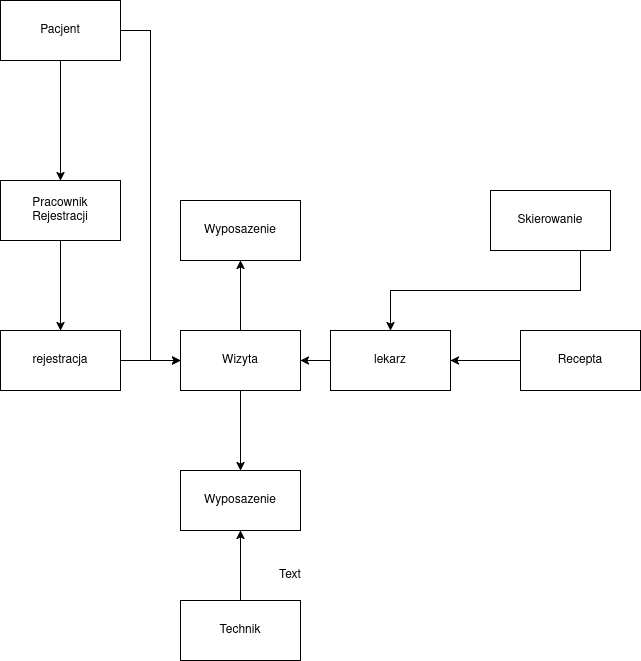
\includegraphics[scale=0.6]{../Diagramy/Klasy/Diagram_konceptualny.png}
\newpage
\subsection{Diagram Obiektów}
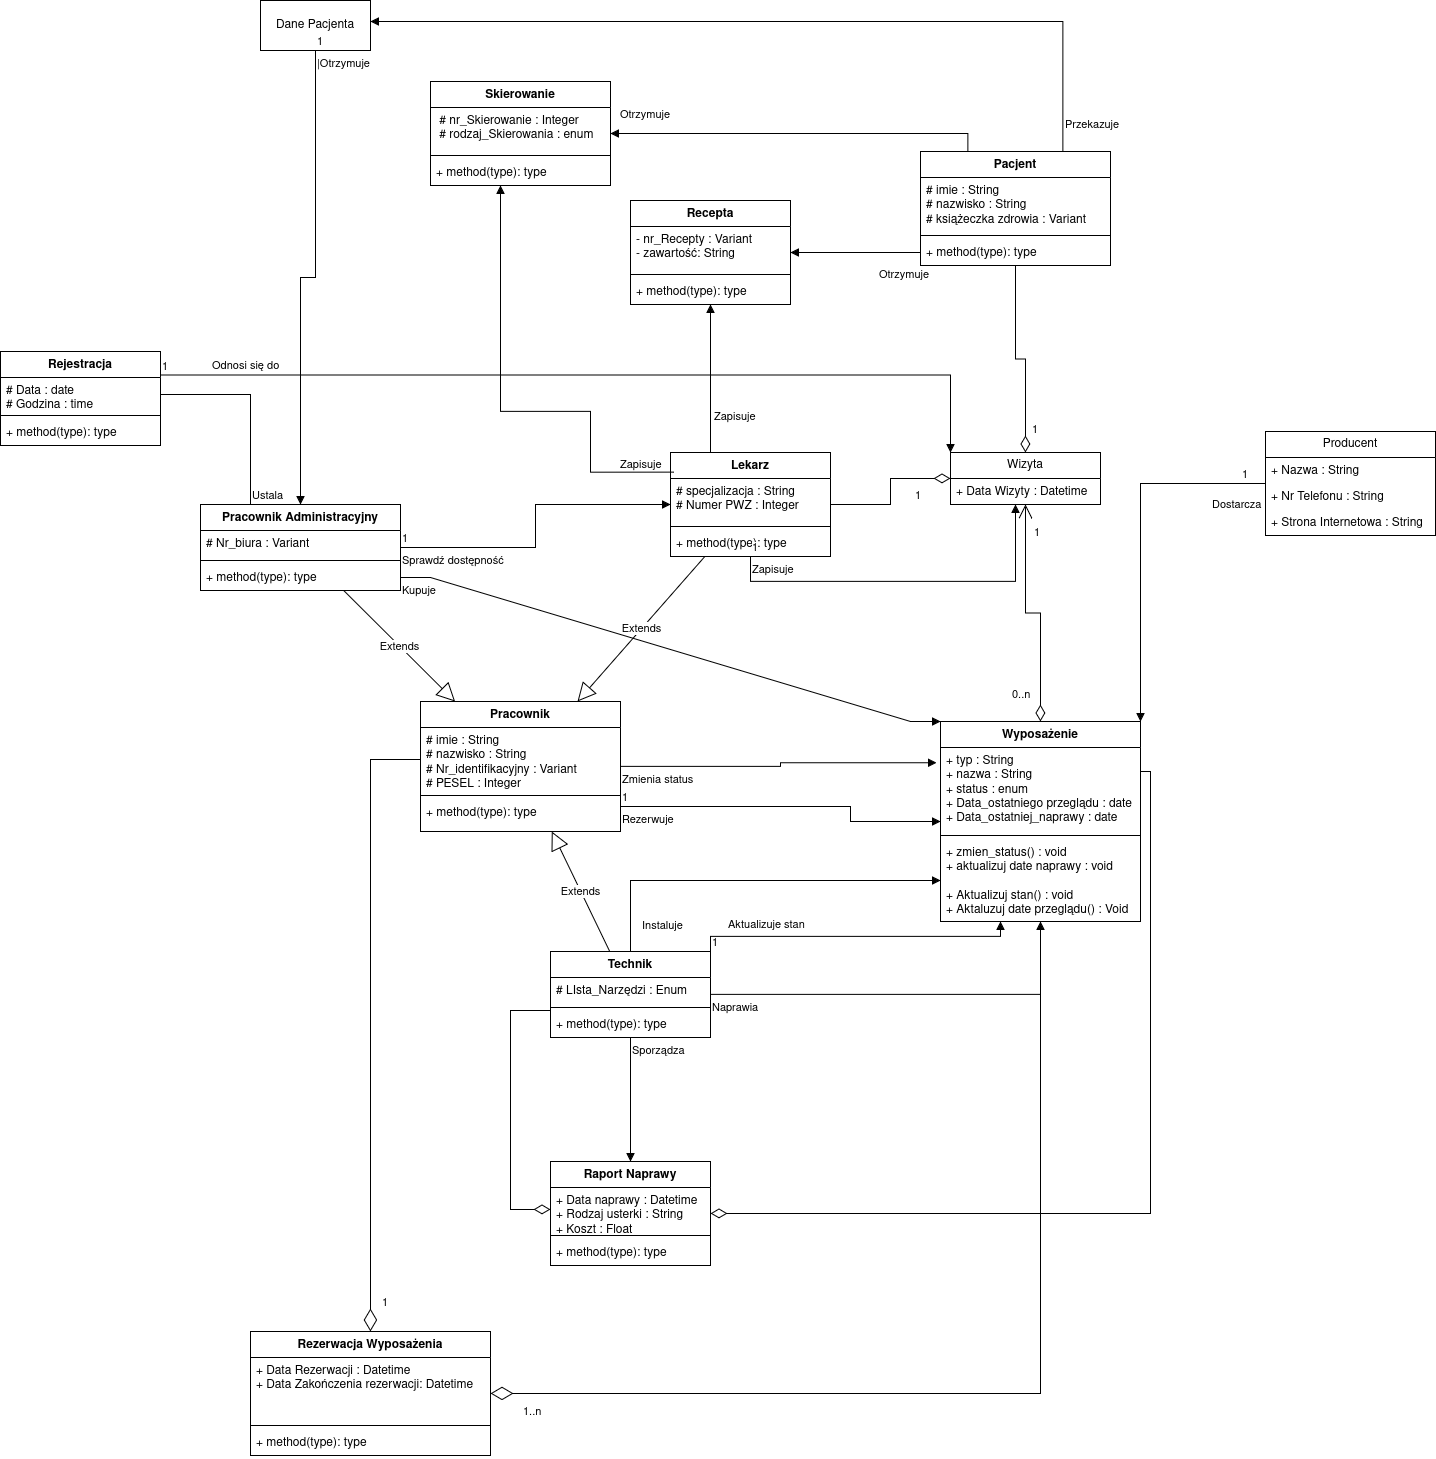
\includegraphics[scale=0.3]{../Diagramy/Klasy/Diagram_klasowy.png}
\newpage
\section{Projektowanie danych}
\subsection{Model bazy danych}
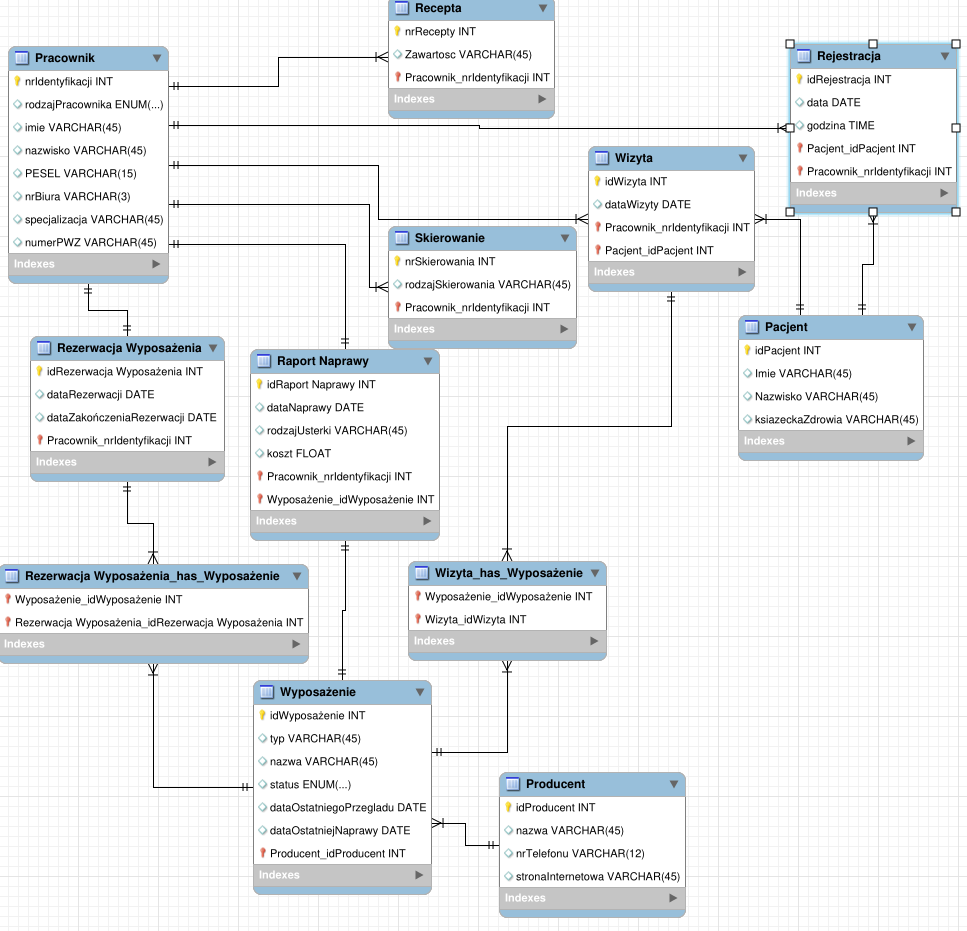
\includegraphics[scale=0.7]{../Diagramy/Baza_danych.png}
\newpage
\section{Projektowanie Interfejsu użytkownika}
\subsection{Menu}
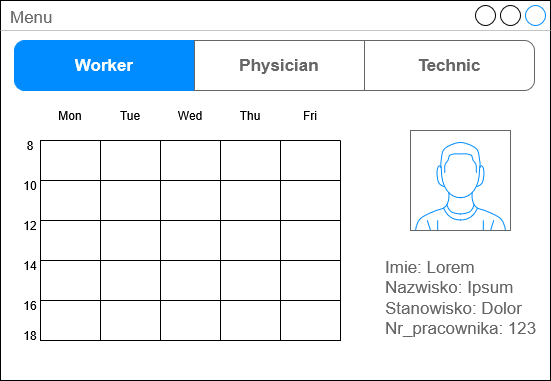
\includegraphics[scale=0.9]{../UI Mock-Up/menu.drawio.png}
\subsection{Login}
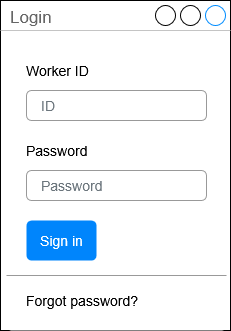
\includegraphics[scale=1]{../UI Mock-Up/Login.drawio.png}
\subsection{Dodanie Wyposażenia}
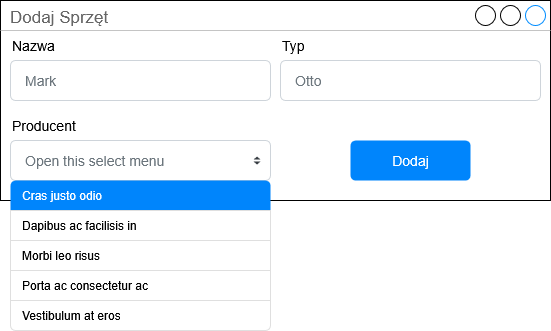
\includegraphics[scale=0.9]{../UI Mock-Up/Dodawanie wyp.drawio.png}
\subsection{Sprawdzanie dostępności}
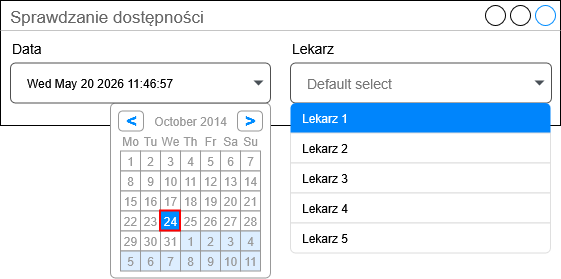
\includegraphics[scale=0.8]{../UI Mock-Up/Sprawdzanie dostepnosci.drawio.png}
\newpage
\section{Modelowanie dynamiki SI}
	\section*{Diagramy Przypadków Użycia}
	\subsection*{Rejestracja Pacjenta}
	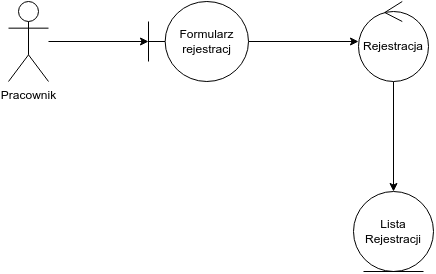
\includegraphics[scale=0.7]{../Diagramy/PU/PU_1.png}
	\subsection*{Sprawdzenie Dostępności}
	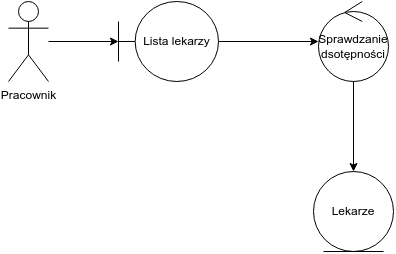
\includegraphics[scale=0.7]{../Diagramy/PU/PU_2.png}
	\subsection*{Zakup nowego wyposażenia}
	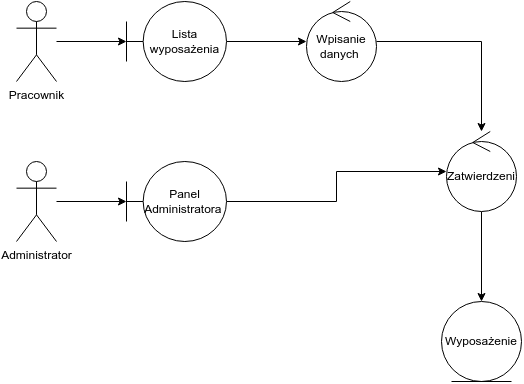
\includegraphics[scale=0.7]{../Diagramy/PU/PU_3.png}
	\subsection*{Instalacja nowego wyposażenia}
	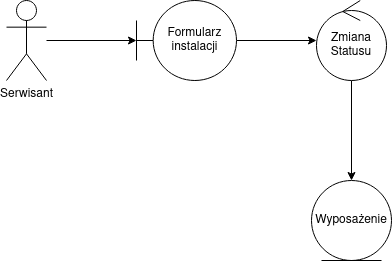
\includegraphics[scale=0.7]{../Diagramy/PU/PU_4.drawio.png}
	\subsection*{Okresowy przegląd wyposażenia}
	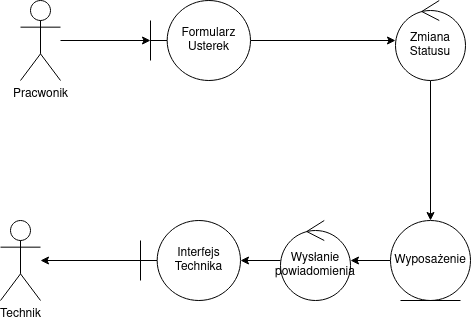
\includegraphics[scale=0.7]{../Diagramy/PU/PU_5.drawio.png}
	\subsection*{Rezerwacja wyposażenia}
	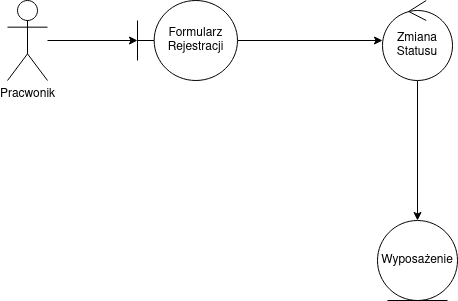
\includegraphics[scale=0.7]{../Diagramy/PU/PU_6.drawio.png}
	\subsection*{Naprawa zepsutego wyposażenia}
	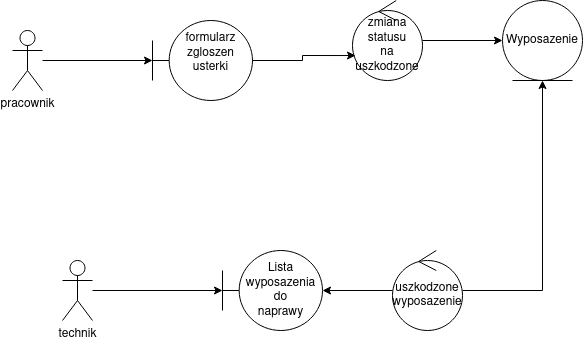
\includegraphics[scale=0.7]{../Diagramy/PU/PU_7.drawio.png}
	\subsection*{Rejestracja pacjenta}
	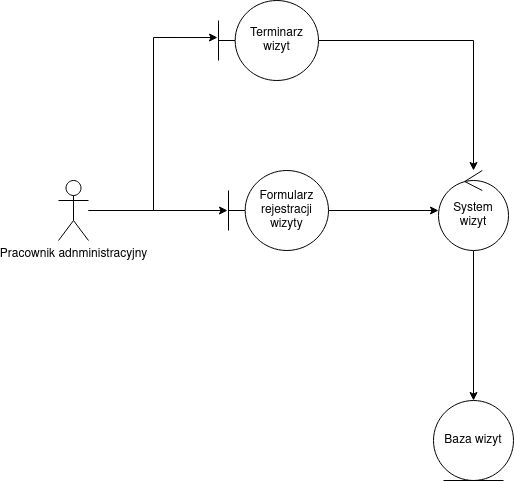
\includegraphics[scale=0.7]{../Diagramy/PU/PU_8.drawio.png}
	\subsection*{Wizyta lekarska}
	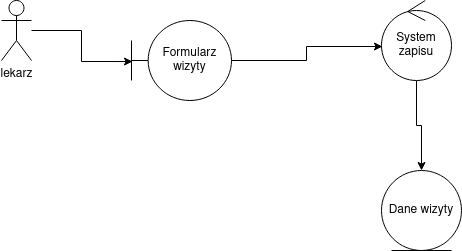
\includegraphics[scale=0.7]{../Diagramy/PU/PU_9.drawio.png}
	\subsection*{Wystawienie recepty}
	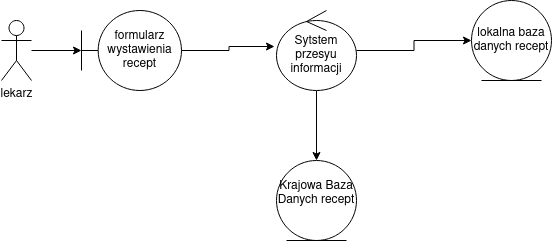
\includegraphics[scale=0.7]{../Diagramy/PU/PU_10.drawio.png}
	\subsection*{Wystawienie Skierowania}
	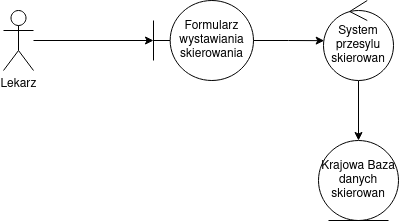
\includegraphics[scale=0.7]{../Diagramy/PU/PU_11.drawio.png}
\newpage
\section{Praca Zespołowa}
\subsection{Wykaz podziału prac}
Podział pracy był równomierny obaj byliśmy zaangażowani nad każdym diagramem dyskutowaliśmy razem i omawialiśmy go a po dyskusji przystępowaliśmy do zrobienia go
Pracowaliśmy regularnie razem w bibliotece konsultując się i uzupełniając
\subsection{Użyte narzędzia}
\begin{itemize}
\item Draw.io
\item \LaTeX
\item MySQLWorkbench
\end{itemize}
\end{document}